\section{System Architecture}

\subsection{Architectural style}

PizzaHUST adopts a web-based client--server architecture. Its current implementation is best described as a \emph{modular monolith}: one frontend application delivers the user interface, one backend application exposes the business API and core workflow logic, and one relational database stores operational data. In addition, the project includes a separate delivery-mock service used to simulate an external courier platform during development and verification.

This architectural choice is deliberate. The business scope is broad enough to require clear separation between customer ordering, administration, kitchen operations, and external delivery integration, but the overall project remains small enough that splitting the core system into multiple business microservices would add unnecessary deployment, debugging, and coordination overhead. A modular monolith therefore provides a suitable compromise between simplicity and structured separation.

\subsection{Architecture rationale}

The original project constraints strongly influence the architecture:

\begin{itemize}
    \item the system targets a single pizza store rather than a large multi-branch enterprise;
    \item the first release is web-only and focused on a manageable academic MVP;
    \item the development timeline is limited;
    \item the team must support both customer-facing and staff-facing workflows;
    \item integration with a delivery provider is required, but a production provider environment may not always be available during development.
\end{itemize}

Under these constraints, a modular monolith offers several advantages:

\begin{itemize}
    \item business rules remain centralized, which is important for pricing, order-state transitions, and delivery coordination;
    \item frontend and backend teams can work in parallel with a contract-defined API;
    \item deployment remains feasible through a small Docker Compose stack;
    \item external delivery behavior can still be tested realistically by isolating the delivery mock as a separate network service.
\end{itemize}

In other words, PizzaHUST is \emph{not} a microservice platform. The delivery mock is separated only to exercise a real integration boundary; the core business system remains one backend application.

\subsection{Technology stack}

\begingroup
\small
\setlength{\LTpre}{0.4em}
\setlength{\LTpost}{0.8em}
\captionof{table}{Technology stack and architectural role}\label{tab:technology-stack}
\begin{tabular}{L{0.24\linewidth} L{0.70\linewidth}}
\toprule
\textbf{Layer} & \textbf{Technology and architectural role} \\
\midrule
Frontend & Next.js 16.2.4 with React 19.2.5, TypeScript 5.9.3, and Tailwind CSS 4.2.4 for the web UI. \\
Backend & Python 3.12 target with FastAPI for HTTP APIs, Pydantic for data validation, and SQLAlchemy 2.x for ORM-based persistence. \\
Database evolution & Alembic migrations maintain schema history and drift control. \\
Database engine & MySQL 8.4 stores operational business data. \\
API contract & OpenAPI is exported by the backend and used to generate TypeScript API types for the frontend. \\
Testing and quality gates & Ruff, mypy, import-linter, pytest, Vitest, Playwright, ESLint, and build checks are combined in the verification pipeline. \\
Local orchestration & Docker Compose coordinates the development/demo runtime stack. \\
\bottomrule
\end{tabular}
\endgroup

\subsection{Runtime topology}

Figure~\ref{fig:system-architecture} shows the runtime view used for local development and demonstration.

\begin{figure}[htbp]
    \centering
    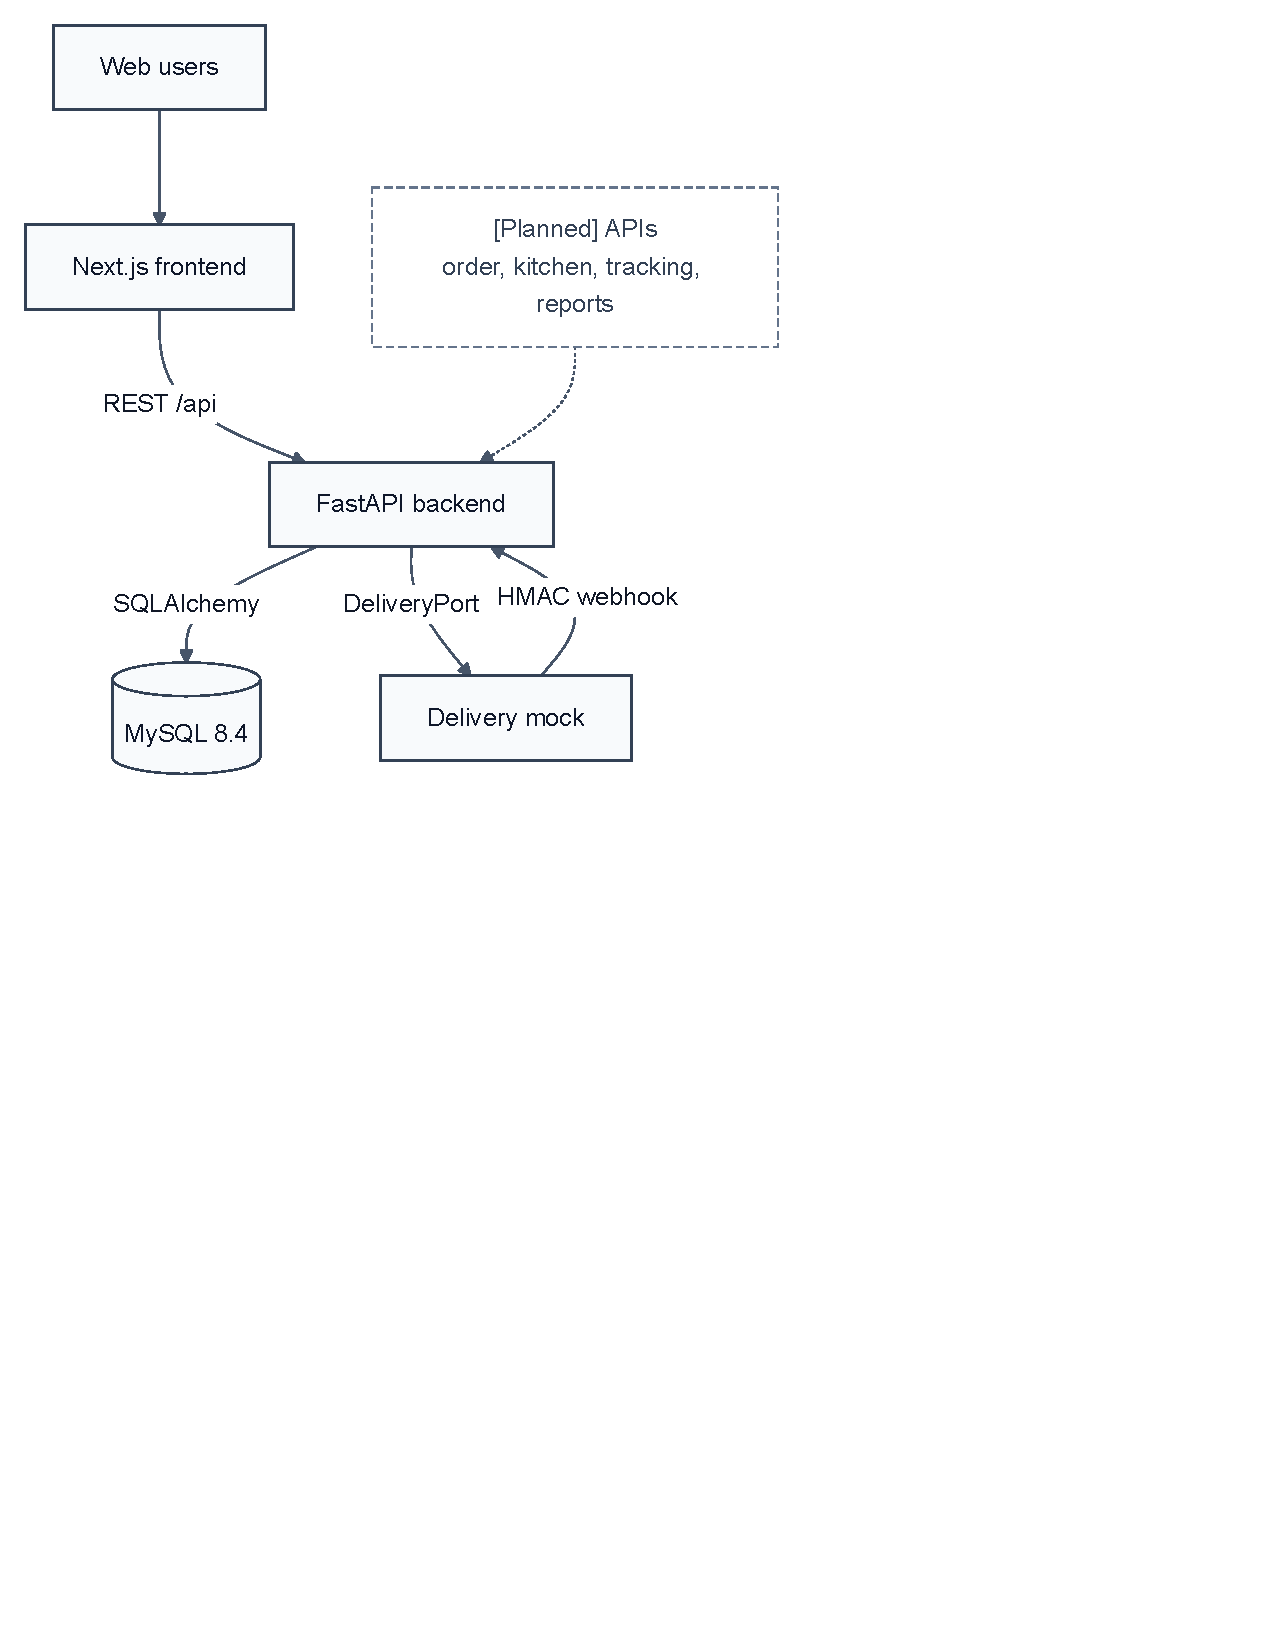
\includegraphics[width=0.86\textwidth,height=0.62\textheight,keepaspectratio,trim=8 410 230 8,clip]{latex_report/figures/system_architecture.pdf}
    \caption{Runtime architecture of PizzaHUST}
    \label{fig:system-architecture}
\end{figure}

The current Compose topology contains four runtime services:

\begin{itemize}
    \item \texttt{mysql}: the primary relational database, exposed internally on port 3306 and mapped to a configurable host port;
    \item \texttt{backend}: the FastAPI application, exposed on port 8000;
    \item \texttt{frontend}: the Next.js application, exposed on port 3000;
    \item \texttt{delivery-mock}: a separate FastAPI service exposed on port 9000 to simulate external courier integration.
\end{itemize}

All four services define health checks in the current development stack. This topology should be understood as a \emph{verified local/demo runtime environment}. The repository also contains infrastructure-oriented deployment assets, but the report should not claim that a production deployment topology has been fully validated solely from these local runtime checks.

\subsection{Backend boundary model}

The backend follows an explicit layered boundary model:

\begin{itemize}
    \item \texttt{app/api/}: HTTP entry points, request validation, response shaping, and orchestration of use-case-level actions;
    \item \texttt{app/domain/}: business rules such as pricing, option validation, combo logic, loyalty rules, service-area validation, and order-state transitions;
    \item \texttt{app/infra/}: persistence, configuration, authentication, and delivery-adapter support;
    \item \texttt{app/seeds/}: development and demo data generation.
\end{itemize}

This boundary model is not only descriptive; it is enforced by import-linter rules. Those rules forbid \texttt{app.domain} from importing API or infrastructure code and forbid \texttt{app.infra} from importing API code. This keeps business rules more testable and reduces coupling across layers.

At application startup, the backend registers routers for configuration, menu browsing, combos, cart behavior, order placement, order history, authentication, loyalty, administrative operations, kitchen operations, and delivery webhooks. This router composition reflects the system's use-case distribution and keeps each functional area addressable within the same API host.

\subsection{Security architecture}

The security model combines session-based authentication, request protection, and integration hardening.

\subsubsection{User authentication and authorization}

PizzaHUST uses Starlette session middleware with signed cookies for authenticated web access. Roles are modeled explicitly as \texttt{customer}, \texttt{admin}, and \texttt{kitchen}. Protected operations rely on role-check dependencies in the backend, while unauthenticated public routes remain available for browsing, quotation preview, and guest-facing actions where appropriate.

Passwords are hashed with Argon2. Mutating operations rely on CSRF protection through token handling, and login/register routes are rate-limited. This is an appropriate match for a browser-based monolithic web application where most state-changing operations originate from the project frontend.

\subsubsection{Delivery-integration security}

The delivery callback path uses HMAC validation and idempotent event recording. Incoming webhook requests must provide a valid signature before any state change is considered. Even for valid requests, repeated or duplicate events are handled safely through a stored webhook-event key. This is important because delivery synchronization is an external integration boundary and must not be trusted in the same way as internal UI actions.

\subsubsection{Request-level observability}

The backend assigns or propagates an \texttt{X-Request-ID} for incoming requests. This supports correlation across logs and responses and gives the API error envelope a stable request reference for troubleshooting.
